\documentclass{article}

\usepackage{iclr2027_conference,times}
\usepackage[T1]{fontenc}
\usepackage{lmodern}
\usepackage{amsmath,amssymb,amsthm,mathtools}
\usepackage{booktabs,microtype,url,xcolor,graphicx}
\usepackage[colorlinks=true,allcolors=blue]{hyperref}

\newtheorem{theorem}{Theorem}
\newtheorem{lemma}[theorem]{Lemma}
\newtheorem{proposition}[theorem]{Proposition}
\newtheorem{corollary}[theorem]{Corollary}
\theoremstyle{remark}
\newtheorem{remark}[theorem]{Remark}
\newtheorem{example}[theorem]{Example}

\newcommand{\E}{\mathbb E}
\newcommand{\Prb}{\mathbb P}
\newcommand{\cL}{\mathcal L}
\newcommand{\cN}{\mathcal N}
\newcommand{\eps}{\varepsilon}
\newcommand{\OPT}{\operatorname{OPT}}
\newcommand{\rank}{\operatorname{rank}}
\newcommand{\tr}{\operatorname{tr}}
\newcommand{\sym}{\operatorname{sym}}
\newcommand{\wtO}{\widetilde O}
\newcommand{\1}{\mathbf 1}

\title{Spectral Fibers for Pure-Relative Matrix Learning and Hessian Correction}
\author{\textbf{Pahan Dewasurendra} \\ Johns Hopkins University}

\hypersetup{pdftitle={Spectral Fibers for Pure-Relative Matrix Learning and Hessian Correction},pdfauthor={Pahan Dewasurendra},pdfkeywords={spectral, fibers, pure-relative, matrix, learning, hessian, correction, large, curvature},pdfsubject={preprint}}
\begin{document}
\maketitle

\begin{abstract}
Large curvature matrices can be applied to vectors long before they can be materialized.  Given products with $A$ and $A^\top$, we study its best Frobenius approximation from an arbitrary known $q$-dimensional linear matrix family.  Classical matrix probing regresses a prescribed dictionary but needs conditioning and high-numerical-rank assumptions.  The recent worst-case theory achieves roughly $\sqrt q$ queries, but only a $(3+\eps)$ approximation with an additive error floor, and leaves pure relative error open.  We resolve this problem with a nonadaptive polynomial-time algorithm.  It returns $\widehat B$ satisfying \[ \|A-\widehat B\|_F^2\le(1+\eps) \min_{B\in\cL}\|A-B\|_F^2 \] using $\wtO(\sqrt{q/\eps})$ products.  The mechanism spectrally splits the known family, measures selected row and column fibers exactly, and regresses only the doubly projected residual.  We also give an affine-baseline form suited to preconditioning.  On a 5,770-dimensional CIFAR-10 last-layer Hessian over frozen MobileNetV3 features, 48 products recover a historical non-Kronecker correction to 0.38\% excess over its family oracle.  Unprojected probing still has 0.43\% excess at 128 products.  At a matched 48-product budget, the reduction repeats by factors of 2.4--4.4 across three independently built dictionaries.  The correction lowers median PCG iterations from 186 for K-FAC and 171 for EK-FAC to 152.  Finally, an adaptive $\Omega(\sqrt{q/\eps})$ lower bound shows that the query law is minimax sharp up to logarithms for $q\ge C/\eps$.
\end{abstract}

\section{Introduction}

Matrix-vector products are a natural interface to large operators.  Automatic differentiation provides Hessian-vector products without materializing a Hessian \citep{pearlmutter1994hessian}.  Scientific simulators apply discretized solution operators whose entries are unavailable.  Operator learning and preconditioning likewise begin with a black-box action and seek a compact surrogate \citep{boulle2024operator,boulle2024adjoint}.  In all of these settings, the number of products can dominate every other cost.

Curvature approximation makes this interface concrete in machine learning. K-FAC replaces a layerwise Fisher or generalized Gauss--Newton block by a Kronecker product \citep{martens2015kfac}.  EK-FAC corrects its eigenvalues while retaining the Kronecker eigenbasis \citep{george2018ekfac}.  Curvature approximation error can matter for inverse-Hessian products \citep{hong2025better,wang2025astra}.  A small reusable correction learned from Hessian-vector products is therefore attractive when many linear systems or influence queries share the same curvature matrix.

We consider the following basic problem.  An unknown $A\in\mathbb R^{n_1\times n_2}$ is accessible through queries $x\mapsto Ax$ and $y\mapsto A^\top y$.  A known linear family $\cL\subseteq\mathbb R^{n_1\times n_2}$ has dimension $q$.  The goal is to return $\widehat B\in\cL$ with
\begin{equation}
 \|A-\widehat B\|_F\le(1+\eps)
 \min_{B\in\cL}\|A-B\|_F.
 \label{eq:goal}
\end{equation}
The family can encode a sparsity pattern, band structure, block model, a linear operator dictionary, or a structured curvature surrogate.

This regression viewpoint has a classical predecessor.  Matrix probing fits a known dictionary from random products and has produced effective scientific preconditioners \citep{chiu2012probing,demanet2012wave}.  Its guarantees require a well-conditioned dictionary Gram matrix and high numerical rank for each basis element.  Its perturbation bound is spectral and relative to an assumed dictionary expansion.  It does not control Frobenius error relative to the best member of an arbitrary supplied family.  We use unprojected Gaussian probing as the classical baseline, not as a new method.

There is a sharp worst-case tension between approximation quality and query complexity.  One-sided subspace sketches give pure relative error with $O(q/\eps)$ products \citep{ahle2020oblivious,chen2019active,amsel2026query}.  The first general two-sided theory gives a nearly quadratic improvement in $q$, but its guarantee for a linear family is \[ \|A-\widetilde B\|_F \le(3+\eps)\min_{B\in\cL}\|A-B\|_F+\alpha\|A\|_F. \] It relies on a cover, adapts its right queries, and has runtime proportional to the cover.  Amsel et al. explicitly conjecture that roughly $\sqrt q/\operatorname{poly}(\eps)$ queries suffice for pure $(1+\eps)$ error and state that a different approach appears necessary \citep{amsel2026query}.

Very recent work nearly characterizes fixed coordinate-sparsity families by a peeling parameter called degeneracy, then explicitly asks for a simple parameter for general linear families \citep{musco2026instance}.  Our residual partial trace supplies a basis-invariant upper-bound parameter for arbitrary linear families.  The two profiles are complementary: degeneracy can be sharper for coordinate patterns, while the spectral profile applies to dense overlapping dictionaries.

We prove that conjecture with the sharp accuracy dependence.  The result is stronger than \eqref{eq:goal} because it controls squared error.

\begin{table}[t]
\centering
\small
\begin{tabular}{@{}llll@{}}
\toprule
Method & query count & guarantee & query pattern \\
\midrule
One-sided or bilinear sketch
& $O(q/\eps)$ & pure $1+\eps$ & nonadaptive \\
\citet{amsel2026query}
& $\wtO(\sqrt{q\log(1/\alpha)}/\eps^2)$
& $3+\eps$ plus $\alpha\|A\|_F$ & adaptive right \\
This work
& $\wtO(\sqrt{q/\eps})$ & pure squared $1+\eps$ & nonadaptive \\
\bottomrule
\end{tabular}
\caption{Worst-case query guarantees for a $q$-dimensional linear family.
Logarithmic confidence factors are suppressed.}
\label{tab:comparison}
\end{table}

\begin{theorem}[Universal pure relative error, informal]
\label{thm:intro-upper}
For every known $q$-dimensional linear matrix family, there is a nonadaptive polynomial-time algorithm that uses \[ \wtO\!\left(\sqrt{q/\eps}\log(1/\delta)\right) \] products with $A$ and $A^\top$ and, with probability at least $1-\delta$, returns $\widehat B\in\cL$ such that \[ \|A-\widehat B\|_F^2\le(1+\eps) \min_{B\in\cL}\|A-B\|_F^2. \] The query count is also at most $\min\{n_1,n_2\}$ by deterministic recovery.
\end{theorem}

The proof introduces a family-side analogue of leverage.  Choose a Frobenius-orthonormal basis $P_1,\ldots,P_q$ of $\cL$ and form
\begin{equation}
 K_L=\sum_{i=1}^qP_iP_i^\top,
 \qquad \tr K_L=q.
 \label{eq:partial-trace-intro}
\end{equation}
The eigenvalues of $K_L$ measure how strongly the whole family concentrates in an output direction.  For a threshold $\tau$, every eigenvector above $\tau$ is queried exactly from the left.  There are at most $q/\tau$ such vectors.  On their orthogonal complement, the family has aggregate leverage at most $\tau$, so $O(\tau/\eps)$ Gaussian right queries suffice for regression.  Balancing the costs at $\tau=\sqrt{q\eps}$ yields $\sqrt{q/\eps}$.

This split has two less obvious properties.  First, the exact and random pieces sum to the full Frobenius objective in expectation.  There is no bias and no covering radius.  Second, if $B_\star$ is the orthogonal projection of $A$ onto $\cL$, then $A-B_\star\perp\cL$.  Estimation error is therefore added in squares, so coefficient accuracy $\sqrt\eps$ gives approximation factor $1+\eps$.  This is the source of the square-root accuracy law.

The upper bound cannot be improved in general, even by adaptive queries.

\begin{theorem}[Matching lower bound, informal]
\label{thm:intro-lower}
There are universal constants $c,C,\eps_0>0$ such that, for every $0<\eps<\eps_0$ and $q\ge C/\eps$, some $q$-dimensional linear family and a distribution on symmetric targets require at least $c\sqrt{q/\eps}$ possibly adaptive products to achieve $(1+\eps)$ relative error with constant probability.
\end{theorem}

The reduction uses the sharp fixed-sparsity lower bound of \citet{amsel2026fixed}.  Its hard pattern has $s$ entries per row in dimension $d\asymp s/\eps$.  The pattern is a linear family of dimension $q\asymp ds\asymp s^2/\eps$, while its lower bound is $s/\eps\asymp\sqrt{q/\eps}$.  Padding gives every prescribed $q$ in the stated regime.  Since the hard target is symmetric, transpose products reveal no new information.

We then test the instance mechanism on deep curvature rather than a synthetic operator.  We fit a linear classification head over frozen ImageNet-pretrained MobileNetV3-Small features and correct its target K-FAC matrix using a family of historical non-Kronecker deviations built from disjoint reference examples. Across three independent dictionaries, spectral fibers at 48 target products have 0.24--0.40\% normalized excess over the exact family projection, compared with 0.95--1.11\% for Gaussian probing at the same budget.  On the main dictionary, 48 fiber products also improve on 128 Gaussian products.  The learned correction is reusable across right-hand sides and reduces PCG iterations below K-FAC, EK-FAC, Jacobi, and no preconditioner on this problem.

\paragraph{Contributions.}
Our main contributions are:

\begin{enumerate}
\item a pure-relative, nonadaptive, polynomial-time algorithm for every linear
matrix family, resolving the open problem of \citet{amsel2026query}
\item an instance-dependent query bound governed by the partial trace after
arbitrary exact row and column fibers are removed
\item a self-adjoint and affine-baseline specialization in which products learn
a correction to an available structured approximation
\item a 5,770-dimensional deep-feature Hessian study with disjoint historical
and target data, matched query budgets, K-FAC and EK-FAC baselines, and three independent dictionaries
\item a proof based on exact population geometry, Gaussian-series covariance
control, and a residual cross-term bound that avoids discretizing $\cL$
\item a matching adaptive lower bound in the regime $q\ge C/\eps$
\end{enumerate}

\section{Spectral fiber regression}
\label{sec:algorithm}

\paragraph{Model.}
A right query chooses $x\in\mathbb R^{n_2}$ and observes $Ax$.  A left query chooses $y\in\mathbb R^{n_1}$ and observes $A^\top y$.  All queries in our algorithm are fixed before observing any response.  Products with $A$ and $A^\top$ each have unit cost.  Computation involving the known family is free in the query model, although our procedure is polynomial time.

Let $P_1,\ldots,P_q$ be a Frobenius-orthonormal basis of $\cL$.  Choose orthonormal $Y\in\mathbb R^{n_1\times r_L}$ and $X\in\mathbb R^{n_2\times r_R}$ using only this known basis.  Write \[ H_L=YY^\top,\quad H_R=XX^\top,\quad \Pi_L=I-H_L,\quad \Pi_R=I-H_R. \] We query $A^\top Y$ and $AX$ exactly, then draw independent $g_1,\ldots,g_m\sim N(0,I_{n_2})$ and query $A\Pi_Rg_j$.  The output is
\begin{equation}
 \widehat B\in\arg\min_{B\in\cL}\left\{
 \|Y^\top(A-B)\|_F^2+\|\Pi_L(A-B)X\|_F^2+
 \frac1m\sum_{j=1}^m\|\Pi_L(A-B)\Pi_Rg_j\|_2^2
 \right\}.
 \label{eq:estimator}
\end{equation}
This is ordinary least squares in $q$ coefficients.  We call its exact observations \emph{fibers}.  All $r_L+r_R+m$ queries are nonadaptive.

\paragraph{Exact population identity.}
For every matrix $D$,
\begin{equation}
 \|Y^\top D\|_F^2+\|\Pi_LDX\|_F^2+
 \E\|\Pi_LD\Pi_Rg\|_2^2=\|D\|_F^2.
 \label{eq:population}
\end{equation}
Indeed, the three terms are the orthogonal blocks $H_LD$, $\Pi_LDH_R$, and $\Pi_LD\Pi_R$.  Thus \eqref{eq:estimator} has no bias or covering radius.

Define the residual basis and its two covariance matrices by
\begin{equation}
 R_i=\Pi_LP_i\Pi_R,\qquad
 \Gamma=\sum_iR_iR_i^\top,\qquad
 G=[\langle R_i,R_k\rangle_F]_{i,k}.
 \label{eq:residual-profile}
\end{equation}
Set $\gamma=\|\Gamma\|$, $\beta=\|G\|$, and $\sigma^2=\max\{\gamma,\beta\}$.  These quantities are basis invariant.  They measure only the family left after the selected fibers have been removed.

\section{Upper and lower query laws}
\label{sec:results}

The logarithmic term below separates concentration from accuracy.  Let \[ \Lambda(\sigma)=\sigma^2\log(2q) \log\!\bigl(2(n_1+q)(1+\sigma^2)\log(2q)\bigr). \]

\begin{theorem}[Residual-family upper bound]
\label{thm:instance}
There is a universal constant $C$ with the following property.  Fix $0<\eps<1$ and any projectors $H_L,H_R$ chosen from the known family.  If
\begin{equation}
 m\ge 1\vee C\left(\frac{\gamma}{\eps}+\Lambda(\sigma)\right),
 \label{eq:m-condition}
\end{equation}
then \eqref{eq:estimator} uses $r_L+r_R+m$ queries and, with probability at least $4/5$, satisfies \[ \|A-\widehat B\|_F^2\le(1+\eps) \min_{B\in\cL}\|A-B\|_F^2. \] If every $R_i=0$, take $m=0$ and the exact fibers return the Frobenius projection deterministically.  Otherwise, reusing the exact fibers and repeating only the random batch $O(\log(1/\delta))$ times raises success to $1-\delta$ without knowing the optimum.
\end{theorem}

The one-projector spectral rule is an immediate specialization.  The partial trace $K_L=\sum_iP_iP_i^\top$ is basis independent and has trace $q$.  For $\tau>0$, let $Y$ contain its eigenvectors above $\tau$, take $X$ empty, and write $H_L=YY^\top$.  Then
\begin{equation}
 r_L\le q/\tau,\qquad \Gamma=\Pi_LK_L\Pi_L\preceq\tau I,
 \qquad \beta\le1.
 \label{eq:spectral-split}
\end{equation}
The transpose construction uses $K_R=\sum_iP_i^\top P_i$.

\begin{corollary}[Universal query complexity]
\label{cor:universal}
For every $q$-dimensional linear matrix family and $0<\eps,\delta<1$, pure relative error is achievable with
\begin{equation}
 \min\left\{n_1,n_2,
 \wtO\!\left(\sqrt{q/\eps}\log(1/\delta)\right)\right\}
 \label{eq:universal-q}
\end{equation}
queries.
\end{corollary}

\begin{proof}
Choose $\tau=\sqrt{q\eps}$.  By \eqref{eq:spectral-split}, $r_L\le\sqrt{q/\eps}$, and $\tau/\eps=\sqrt{q/\eps}$.  If $\tau\ge1$, the concentration term $\Lambda(\sigma)$ is at most this scale times logarithms.  If $\tau<1$, the same holds because $\sqrt{q/\eps}\ge1$.  Querying every column or every row recovers $A$ deterministically and gives the ambient cap.
\end{proof}

The pure guarantee has a useful endpoint.  If $A\in\cL$, then the optimum is zero, and the algorithm recovers $A$ exactly on its success event.

\begin{corollary}[Self-adjoint residual profile]
\label{cor:self-adjoint}
Suppose $A$ and every member of $\cL$ are symmetric.  For any $H=YY^\top$, the $r=\rank(H)$ ordinary products $AY$ reveal both exact blocks. With $\Pi=I-H$ and $R_i=\Pi P_i\Pi$, Theorem~\ref{thm:instance} therefore needs only \[ r+\left[1\vee\wtO\!\left(\frac{\|\sum_iR_i^2\|}{\eps} +\max\{\|\sum_iR_i^2\|,\|G\|\}\right)\right] \] Hessian-vector products.  If all $R_i=0$, exactly $r$ products suffice.
\end{corollary}

This is more than a notational saving.  Exact products on $Y$ remove the family on both sides before regression.  A single hub direction, for example, removes every incident interaction in a symmetric arrowhead family.

\begin{corollary}[Affine baseline]
\label{cor:affine}
Let $B_0$ be any known matrix and let the hypothesis class be $B_0+\cL$.  Every upper bound above applies unchanged to this affine class by replacing each response with $(A-B_0)x$ or $(A-B_0)^\top y$.  In particular, the query complexity depends on $\cL$ and not on the rank or norm of $B_0$.
\end{corollary}

For a known positive-definite baseline $P_0$ and target Hessian $H$, take $A=P_0^{-1/2}HP_0^{-1/2}$ and $B_0=I$.  Each product with $A-I$ needs one HVP and known baseline transforms.  The learned correction can be reused for every right-hand side.  The following elementary bound records when Frobenius recovery certifies a useful preconditioner.

\begin{proposition}[Stable preconditioning after clipping]
\label{prop:preconditioning}
Let $A=A^\top\succeq\mu I$ and let $\widetilde A$ be symmetric.  Denote the Frobenius projection of $\widetilde A$ onto $\{M=M^\top:M\succeq\mu I\}$ by $P$.  If $e=\|A-\widetilde A\|_F<\mu$, then \[ \kappa(P^{-1/2}AP^{-1/2}) \le \frac{1+e/\mu}{1-e/\mu}. \]
\end{proposition}

\begin{proof}
Projection onto a closed convex set is nonexpansive, and $A$ belongs to the set.  Hence $\|A-P\|_F\le e$.  Since $P\succeq\mu I$, $\|P^{-1/2}(A-P)P^{-1/2}\|\le e/\mu$.  The eigenvalues of $P^{-1/2}AP^{-1/2}$ lie in $[1-e/\mu,1+e/\mu]$.
\end{proof}

\begin{theorem}[Adaptive lower bound]
\label{thm:lower}
There are universal constants $c,C,\eps_0>0$ such that the following holds. For every $0<\eps<\eps_0$ and integer $q\ge C/\eps$, there are dimensions, a known $q$-dimensional linear family $\cL$, and a distribution on symmetric targets $A$ such that every randomized algorithm using fewer than $c\sqrt{q/\eps}$ possibly adaptive queries to $A$ and $A^\top$ has \[ \Prb\!\left\{ \|A-\widehat B\|_F\le(1+\eps) \min_{B\in\cL}\|A-B\|_F \right\}\le\frac1{25}. \]
\end{theorem}

Corollary~\ref{cor:universal} and Theorem~\ref{thm:lower} match up to logarithms for $q\ge C/\eps$.  We do not claim a matching lower bound in the small-$q$ endpoint $q<C/\eps$.  The upper theorem uses squared error while the lower theorem uses norm error.  Since $\sqrt{1+\eps}\le1+\eps/2$ and $(1+\eps)^2\le1+3\eps$ for $0<\eps<1$, constant rescaling of $\eps$ makes the two formulations equivalent here.

\subsection{What the spectrum means}

\begin{example}[Fixed sparsity]
Suppose $\cL$ contains matrices supported on a fixed pattern, and row $a$ has $d_a$ allowed entries.  For the coordinate basis, $K_L=\operatorname{diag}(d_1,\ldots,d_{n_1})$.  Theorem~\ref{thm:instance} gives, up to logarithms,
\begin{equation}
 \min_{\tau>0}\left\{\#\{a:d_a>\tau\}+\frac{\tau}{\eps}\right\}.
 \label{eq:sparsity-profile}
\end{equation}
Rows above the threshold are read exactly.  The others are fit from common Gaussian probes.  If every $d_a\le s$, choosing $\tau=s$ recovers the known $O(s/\eps)$ law of \citet{amsel2026fixed}.  Degeneracy peeling can be sharper for some coordinate patterns, including arrowheads \citep{musco2026instance}. Our two-projector profile instead applies unchanged to noncoordinate linear combinations and can remove dense row and column fibers simultaneously.
\end{example}

\begin{example}[Concentrated and diffuse families]
If all matrices in $\cL$ are supported on $r$ output directions, then those directions can be measured with $r$ left products, and the random component may vanish.  At the opposite extreme, a diffuse family has small $\|K_L\|$.  It needs no exact fibers and reduces to Gaussian regression.  The algorithm continuously interpolates between these cases.
\end{example}

For implicit Hessians, Corollary~\ref{cor:self-adjoint} approximates the best member of any known linear curvature dictionary.  The approximation family need not be coordinate sparse or positive semidefinite.  Positive-definite clipping may be applied afterward when the estimate is used as a preconditioner.

\begin{proposition}[An exact side-information separation]
\label{prop:side-separation}
For every $q$, there is a $q$-dimensional linear family whose Frobenius projection can be recovered from one left query for every target, while any right-only algorithm needs at least $q$ queries to guarantee pure relative error.  The transpose statement also holds.
\end{proposition}

\begin{proof}
Let $n_1\ge1$, $n_2=q$, and $\cL=\{e_1v^\top:v\in\mathbb R^q\}$.  The projection of $A$ onto $\cL$ is $e_1(e_1^\top A)$, which the left query $A^\top e_1$ reveals exactly.  For a target already in $\cL$, every right query returns only one informative scalar, $v^\top x$.  Pure relative error requires exact recovery because $\OPT=0$. Fewer than $q$ scalar linear measurements cannot identify every $v\in\mathbb R^q$, even adaptively.  Transposing the construction exchanges the two sides.
\end{proof}

Here $K_L=qe_1e_1^\top$, so the spectral algorithm discovers the one-query solution directly.  The example also explains why a trace-only dimension bound cannot describe instance difficulty without its leverage spectrum.

Structure-specific recovery can be better than the universal bound.  For example, circulant and Toeplitz matrices admit constant-query exact procedures \citep{halikias2024structured,otto2023generic}.  Our result is a worst-case guarantee for an arbitrary supplied basis, not a replacement for algebraic algorithms tailored to one family.

\section{Why the estimator works}
\label{sec:proof}

We give the proof architecture here and defer concentration constants to Appendix~\ref{app:concentration}.  For $g\sim N(0,I)$ define $F_g\in\mathbb R^{n_1\times q}$ by \[ F_gc=\sum_{i=1}^qc_iR_ig. \] Its population Gram matrix is $G$ from \eqref{eq:residual-profile}.  The exact-fiber Gram matrix is exactly $I-G$ by orthonormality of the $P_i$.

\subsection{The Hessian sees only low leverage}

Write $F_g=\sum_{b=1}^{n_2}g_bC_b$, where column $i$ of $C_b$ is $R_ie_b$. The two variance matrices of this rectangular Gaussian series satisfy
\begin{equation}
 \sum_bC_bC_b^\top=\sum_iR_iR_i^\top=\Gamma\preceq\gamma I,
 \qquad
 \sum_bC_b^\top C_b=G\preceq\beta I.
 \label{eq:series-variance}
\end{equation}
The rectangular Gaussian-series inequality therefore gives \[ \Prb\{\|F_g\|\ge t\} \le(n_1+q)\exp\!\left[-\frac{t^2}{2\sigma^2}\right] \] \citep{tropp2015matrix}.  Truncating this tail and applying matrix Bernstein shows that $m\gtrsim\Lambda(\sigma)$ implies
\begin{equation}
 \left\|\frac1m\sum_{j=1}^mF_{g_j}^\top F_{g_j}-G\right\|\le\frac18.
 \label{eq:hessian-conc}
\end{equation}
Adding the deterministic Gram $I-G$ puts the empirical Hessian between $7I/8$ and $9I/8$.  This is the only subspace embedding needed in the proof.

\subsection{The residual noise is smaller by a square root}

Let $B_\star$ be the Frobenius projection of $A$ onto $\cL$ and set $N=A-B_\star$.  Then $N\perp\cL$.  At $B_\star$, the deterministic gradient and the mean random gradient cancel:
\begin{equation}
 \langle H_LP_i,H_LN\rangle_F+
 \langle\Pi_LP_iH_R,\Pi_LNH_R\rangle_F+
 \langle R_i,\Pi_LN\Pi_R\rangle_F
 =\langle P_i,N\rangle_F=0.
 \label{eq:gradient-cancel}
\end{equation}
The empirical normal equations have centered right-hand side $z\in\mathbb R^q$,
\begin{equation}
 z_i=\frac1m\sum_{j=1}^m
 \left(g_j^\top R_i^\top\Pi_LN\Pi_Rg_j
 -\tr(R_i^\top\Pi_LN\Pi_R)\right).
 \label{eq:z}
\end{equation}
Gaussian quadratic-form variance and \eqref{eq:residual-profile} give
\begin{align}
 \E\|z\|_2^2
 &\le\frac2m\sum_i\|R_i^\top\Pi_LN\Pi_R\|_F^2 \\
 &\le\frac{2\gamma}{m}\|N\|_F^2.
 \label{eq:z-bound}
\end{align}
On the Hessian event, the coefficient error is at most a constant times $\|z\|_2$.  Markov's inequality is enough for constant success probability. Thus $m\gtrsim\gamma/\eps$ gives \[ \|\widehat B-B_\star\|_F^2\le\eps\|N\|_F^2. \] Finally, orthogonality gives the exact identity
\begin{equation}
 \|A-\widehat B\|_F^2
 =\|N\|_F^2+\|\widehat B-B_\star\|_F^2,
 \label{eq:pythagorean}
\end{equation}
which proves pure relative error.

The Hessian and $z$ use the same probes.  The proof does not assume they are independent.  It bounds each bad event and takes a union bound.

\section{Deep Hessian correction from historical curvature}
\label{sec:experiments}

\paragraph{Target and baseline.}
We extract 576-dimensional features from an ImageNet-pretrained MobileNetV3-Small on CIFAR-10 \citep{howard2019mobilenet,krizhevsky2009cifar}, freeze the backbone, standardize the features, append a bias, and fit a ten-class linear head on 4,000 examples.  Its accuracy on 1,000 held-out examples is 82.7\%.  If $z_i\in\mathbb R^{577}$ is a feature and $p_i$ is the predicted class distribution, the regularized last-layer Hessian is \[ H=\frac1N\sum_{i=1}^N [\operatorname{diag}(p_i)-p_ip_i^\top]\otimes z_iz_i^\top +10^{-3}I\in\mathbb R^{5770\times5770}. \] The reference and target curvature sets contain 1,500 disjoint head-training examples each.  On the target set, $P_0$ is the usual K-FAC product of the mean class and feature factors, with the same ridge.  We learn a correction to the whitened operator $A=P_0^{-1/2}HP_0^{-1/2}$ as in Corollary~\ref{cor:affine}.  EK-FAC, computed in the K-FAC eigenbasis from the same target examples, is a stronger target-data baseline.

\paragraph{Historical family.}
We retain the nine nonnull class-factor modes and top eight feature-factor modes, giving a fixed 72-dimensional support.  For each of 128 independently sampled 375-example subsets of the reference set, we form its exact reduced curvature minus its own K-FAC approximation.  The Frobenius-orthonormal span of these non-Kronecker deviations has dimension $q=128$.  This family and its spectral profile are frozen before any target HVP.  The offline reference cost is not charged to the target query budget.

We compare self-adjoint spectral fibers with classical unprojected Gaussian probing.  Both regress the same family and each reduced product is implemented by one full target HVP.  The normalized projection excess is \[ \frac{\|\widehat C-C_\star\|_F^2}{\|C_\star\|_F^2}, \qquad C_\star=\operatorname{proj}_{\cL}(A-I). \] The exact 72-product reduced target used to compute $C_\star$ is evaluation only and is never supplied to either estimator.  We report medians over 30 independent query batches.

\begin{figure}[t]
  \centering
  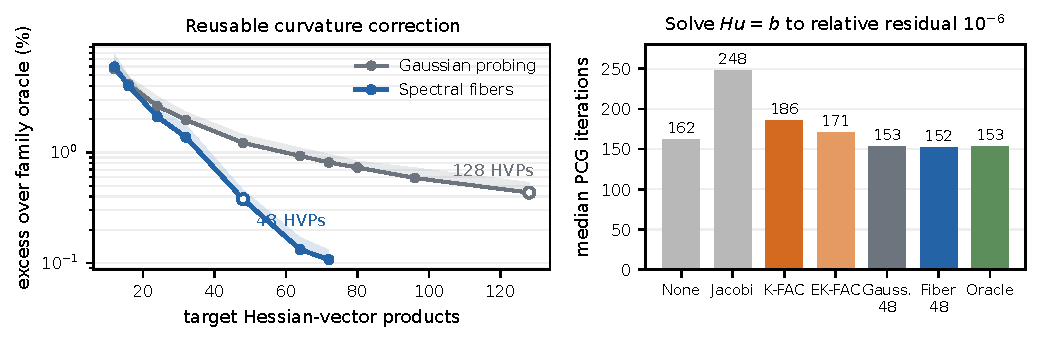
\includegraphics[width=\linewidth]{deep_hessian_study.pdf}
  \caption{Left: normalized excess over the exact historical-family projection.
Lines are medians and bands extend to the 90th percentile.  Fibers at 48 HVPs improve on Gaussian probing at 128 HVPs.  Right: median PCG iterations over ten right-hand sides.  The 48-HVP estimates are median-error trials, not best-case selections.  Bars exclude the one-time 48-HVP fitting cost.}
  \label{fig:deep-hessian}
\end{figure}

At 48 HVPs, fibers have 0.378\% median excess, compared with 1.220\% for Gaussian probing.  Even at 128 HVPs, Gaussian probing has 0.434\% excess.  Thus the family-side spectrum gives a $2.7\times$ product reduction at this fixed accuracy on the main dictionary.  At the matched 48-HVP budget, the advantage repeats for all three additional historical dictionaries on the same data split:

\begin{table}[h]
\centering
\small
\begin{tabular}{@{}rrrr@{}}
\toprule
dictionary seed & fibers, 48 & Gaussian, 48 & Gaussian, 128 \\
\midrule
2027 & 0.378\% & 1.220\% & 0.434\% \\
3    & 0.243\% & 1.081\% & 0.399\% \\
11   & 0.400\% & 0.946\% & 0.367\% \\
29   & 0.268\% & 1.111\% & 0.408\% \\
\bottomrule
\end{tabular}
\caption{Median normalized projection excess.  Only the reference dictionary
and estimator randomness change.}
\label{tab:dictionary-robustness}
\end{table}

Fibers at 48 HVPs improve on Gaussian at 128 HVPs for seeds 2027, 3, and 29. For seed 11, the respective excesses are 0.400\% and 0.367\%, so we do not claim that the $2.7\times$ crossing is uniform over dictionaries.

For the downstream diagnostic, we clip the whitened estimate at $10^{-3}$ and use it with K-FAC as a preconditioner.  No learned estimate is clipped in the reported main trial.  At relative residual $10^{-6}$, median PCG counts are 152 for fibers, 153 for Gaussian probing and the family oracle, 171 for EK-FAC, 186 for K-FAC, 162 without preconditioning, and 248 for Jacobi.  The corresponding 150-step Lanczos Ritz condition estimates are 648, 645, 649, 722, 946, 1,093, and 3,530.  The one-iteration differences among the learned fits and oracle are not meaningful.  Their common improvement shows that the small correction is reusable across solves.  Notably, the family projection explains only 0.20\% of the global whitened residual energy, so we do not claim broad Hessian reconstruction.  It captures directions that improve this solve diagnostic. Counting one HVP per PCG iteration, the median fiber total is $48+152R$ for $R$ right-hand sides, versus $186R$ for K-FAC, $171R$ for EK-FAC, and $162R$ without preconditioning.  The one-time fit therefore amortizes after 2, 3, and 5 solves, respectively, under this accounting. Appendix~\ref{app:numerics} gives all splits, seeds, query accounting, and mechanism checks.

\section{Related work and limitations}
\label{sec:discussion}

\paragraph{Matrix probing and structured queries.}
Classical matrix probing solves a least-squares system whose columns are random products with prescribed basis matrices \citep{chiu2012probing}.  Its scientific applications include wave-Hessian and elliptic preconditioning \citep{chiu2012probing,demanet2012wave}.  The theory depends on dictionary Gram conditioning and high numerical rank of each basis matrix.  Our unprojected baseline is this estimator.  Spectral fibers remove both assumptions and give a best-in-family pure-relative guarantee.

\citet{amsel2026query} initiate the recent worst-case theory for arbitrary matrix families and provide the direct open problem resolved here.  For fixed sparsity, \citet{amsel2026fixed} prove the row-sparsity law used by our lower bound, while \citet{musco2026instance} give a complementary degeneracy-peeling characterization and explicitly leave a parameter for general linear families open.  Structure-specific methods cover Toeplitz and tridiagonal recovery \citep{halikias2024structured,otto2023generic}, HODLR and HSS approximation \citep{chen2024hodlr,amsel2025hss}, adaptive low rank \citep{smith2026adaptive}, and butterfly factorization \citep{persson2026butterfly}.  These nonlinear classes use additional algebraic structure and do not imply the arbitrary-linear-family theorem.  The recent transpose-free lower bounds explain why two-sided access matters in the general nonsymmetric model \citep{halikias2026transpose}.  Scalar bilinear queries are different: Khatri--Rao sketches use $O(q)$ for constant-factor approximation \citep{camano2025structured}.

\paragraph{Curvature and preconditioning.}
K-FAC approximates each layer block by a Kronecker product, while EK-FAC is the Frobenius-optimal diagonal correction in the K-FAC eigenbasis \citep{martens2015kfac,george2018ekfac}.  M-FAC exactly inverts a damped empirical-Fisher low-rank surrogate, and Shampoo accumulates tensor-mode gradient second moments \citep{frantar2021mfac,gupta2018shampoo}.  These methods use different curvature families or gradient statistics and do not regress a best arbitrary-family approximation to a target HVP oracle.  Active probabilistic matrix inference chooses noisy Hessian projections under a Gaussian prior and returns a low-rank posterior mean \citep{deroos2019active}.  ASTRA instead uses EK-FAC to precondition hundreds of stochastic Neumann iterations separately for each inverse-Hessian query \citep{wang2025astra}.  Our correction is learned once from a fixed product batch and then reused.  Projected Hessian Learning uses random HVP supervision inside interatomic-potential training, illustrating another role for product access rather than operator recovery \citep{rodriguez2026projected}.

\paragraph{Variance reduction.}
The high-fiber split is related in spirit to Hutch++, which deflates a leading subspace of the target before stochastic trace estimation \citep{meyer2021hutchpp}.  Partial-trace estimators also use target-dependent deflation \citep{chen2024partial}.  Here the split is computed from the known hypothesis family, and its deterministic and random terms reconstruct an entire Frobenius regression objective.  The target is never spectrally approximated.

\paragraph{Limitations.}
The theorem concerns linear families and Frobenius error.  Nonlinear families, including fixed-rank and many hierarchical models, need different ideas.  The preprocessing can be expensive when the basis itself is large, although it is polynomial and requires no oracle products.  Our lower bound matches the upper law for $q\ge C/\eps$ but leaves the small-$q$ accuracy endpoint open.  Finally, the result is an oracle-complexity theorem.  Wall-clock gains depend on whether products can be batched and on the coefficient solve.  The deep study freezes the backbone and concerns only the last-layer Hessian.  Its historical family is built offline from reference curvature and transfers across one fixed data split.  Scaling the construction to full-network curvature and measuring end-to-end optimization or attribution gains remain open.

\bibliography{references}
\bibliographystyle{iclr2027_conference}

\appendix

\section{Complete covariance proof}
\label{app:concentration}

We prove the concentration statement used in Theorem~\ref{thm:instance}.  The constants are not optimized.

\begin{lemma}[Fiber covariance]
\label{lem:fiber-cov}
Let $F_g=\sum_bg_bC_b\in\mathbb R^{n_1\times q}$ be defined as in Section~\ref{sec:proof}, let $G=\E F_g^\top F_g$, assume $\sigma^2>0$, and set $p=n_1+q$.  For $0<\eta<1/2$, there is a constant $C$ such that \[ m\ge C\sigma^2\log(2q/\eta) \log\!\left(2p(1+\sigma^2)\log(2q/\eta)/\eta\right) \] implies \[ \left\|m^{-1}\sum_{j=1}^mF_{g_j}^\top F_{g_j}-G\right\|\le\frac18 \] with probability at least $1-\eta$.
\end{lemma}

\begin{proof}
Equation~\eqref{eq:series-variance} and the rectangular Gaussian-series bound give
\begin{equation}
 \Prb\{\|F_g\|^2>u\}\le p\exp[-u/(2\sigma^2)].
 \label{eq:gaussian-tail-app}
\end{equation}
Choose \[ L=C_0\sigma^2\log(pm(1+\sigma^2)/\eta),\qquad Z_g=F_g^\top F_g\1\{\|F_g\|^2\le L\}, \] where $C_0$ is a sufficiently large numerical constant.  Integrating \eqref{eq:gaussian-tail-app} gives
\begin{align}
 \E[\|F_g\|^2\1\{\|F_g\|^2>L\}]
 &=L\Prb\{\|F_g\|^2>L\}
   +\int_L^\infty\Prb\{\|F_g\|^2>u\}\,du \\
 &\le p(L+2\sigma^2)e^{-L/(2\sigma^2)}\le\frac1{16}.
 \label{eq:tail-bias}
\end{align}
If $M=\E Z_g$, then
\begin{equation}
 0\preceq G-M\preceq\frac1{16}I.
 \label{eq:trunc-bias}
\end{equation}
Moreover, $0\preceq Z_g\preceq LI$ and $Z_g^2\preceq LZ_g$.  Therefore \[ \E(Z_g-M)^2=\E Z_g^2-M^2\preceq\E Z_g^2\preceq LM\preceq LI. \] Matrix Bernstein yields
\begin{equation}
 \left\|m^{-1}\sum_{j=1}^mZ_{g_j}-M\right\|\le\frac1{16}
 \label{eq:bernstein-app}
\end{equation}
with probability at least $1-\eta/2$ when $m\ge C_1L\log(2q/\eta)$.  The same tail bound and a union bound ensure $Z_{g_j}=F_{g_j}^\top F_{g_j}$ for all $j$ with probability at least $1-\eta/2$.  Combining \eqref{eq:trunc-bias} and \eqref{eq:bernstein-app} proves the claim.  The displayed sufficient condition solves the logarithm containing $m$ after increasing $C$.
\end{proof}

\section{Complete upper-bound proof}
\label{app:upper}

\begin{proof}[Proof of Theorem~\ref{thm:instance}]
Let $B_\star=P_\cL A$ and $N=A-B_\star$.  Write $B_\star=\sum_ic_i^\star P_i$ and $\widehat B=\sum_i\widehat c_iP_i$.  By Lemma~\ref{lem:fiber-cov} with $\eta=1/10$, the Hessian $\widehat G$ of \eqref{eq:estimator} obeys
\begin{equation}
 \frac78I\preceq\widehat G\preceq\frac98I
 \label{eq:hessian-app}
\end{equation}
with probability at least $9/10$, provided the concentration term in \eqref{eq:m-condition} holds.

Equation~\eqref{eq:gradient-cancel} shows that the empirical normal equations are \[ \widehat G(\widehat c-c^\star)=z, \] up to an immaterial sign, with $z$ given in \eqref{eq:z}.  For any real matrix $M$ and standard Gaussian $x$, \[ \operatorname{Var}(x^\top Mx) =2\|\sym M\|_F^2\le2\|M\|_F^2. \] Thus \eqref{eq:z-bound} holds.  Markov's inequality gives \[ \|z\|_2^2\le20\gamma\|N\|_F^2/m \] with probability at least $9/10$.  This event need not be independent of \eqref{eq:hessian-app}.  A union bound gives both with probability at least $4/5$.  On their intersection, \[ \|\widehat B-B_\star\|_F^2 =\|\widehat c-c^\star\|_2^2 \le(8/7)^2\|z\|_2^2 \le C_2\gamma\|N\|_F^2/m. \] Taking $m\ge C_2\gamma/\eps$ and using \eqref{eq:pythagorean} proves the base guarantee.

For amplification, reuse the exact fibers and run the random batch independently $R=C_3\log(1/\delta)$ times with excess-error target $\eps/9$.  With probability at least $1-\delta$, more than half the coefficient vectors lie within radius $\sqrt\eps\|N\|_F/3$ of $c^\star$.  Select the candidate with smallest median distance to the others.  Its median distance is at most twice that radius.  The selected candidate's median ball intersects the majority of good candidates, so it lies within three radii of $c^\star$.  Equation \eqref{eq:pythagorean} completes the amplified claim.
\end{proof}

\begin{proof}[Proof of Corollary~\ref{cor:self-adjoint}]
Set $H_L=H_R=H$ in Theorem~\ref{thm:instance}.  Symmetry gives $Y^\top A=(AY)^\top$, so the same $r$ products reveal both exact terms $\|Y^\top(A-B)\|_F^2$ and $\|\Pi(A-B)Y\|_F^2$.  The random queries use $\Pi g_j$, and their residual basis is $R_i=\Pi P_i\Pi$.  The theorem now gives the displayed profile.  If every $R_i=0$, the exact-fiber Gram is $I$ by \eqref{eq:population}, so its least-squares solution is the Frobenius projection without random queries.
\end{proof}

\section{Lower-bound reduction}
\label{app:lower}

\begin{proof}[Proof of Theorem~\ref{thm:lower}]
Theorem 2 of \citet{amsel2026fixed} gives constants with the following property.  For every integer $s\ge1$ and sufficiently small $\eps$, there is a symmetric Wishart hard distribution in dimension $d=\Theta(s/\eps)$.  For every fixed sparsity pattern $S$ having between $\gamma s$ and $s$ entries in every row and column, any possibly adaptive algorithm that uses fewer than $c_0s/\eps$ matvecs fails to return an $S$-supported matrix with $(1+\eps)$ relative error with probability at least $24/25$.  Their proof specifies the displayed relation between $d$, $s$, and $\eps$.  Since the target is symmetric, allowing products with the transpose does not strengthen the oracle.

Choose an $s$-regular pattern.  Its supported matrices form a linear subspace $\cL_0$ of dimension \[ q_0=ds=\Theta(s^2/\eps). \] The lower bound is therefore \[ \Omega(s/\eps)=\Omega(\sqrt{q_0/\eps}). \]

Now fix $q\ge C/\eps$.  Write the cited dimension relation as $a s/\eps\le d\le b s/\eps$ for universal $a,b>0$.  Choose $s=\lfloor\sqrt{q\eps/(2b)}\rfloor$.  Increasing $C$ ensures $s\ge2$, and therefore $q_0=ds\le q$ while $q_0\ge c_1q$.  Integer rounding only changes universal constants.  Enlarge the ambient matrix by a disjoint block and add $q-q_0$ coordinate basis matrices supported in that block.  Call the resulting $q$-dimensional family $\cL$ and embed the hard target as $A=\operatorname{diag}(A_0,0)$.

Every query to $A$ can be simulated by one query to $A_0$.  If $\widehat B\in\cL$ achieves relative error for $A$, its restriction $\widehat B_0\in\cL_0$ satisfies \[ \|A_0-\widehat B_0\|_F \le\|A-\widehat B\|_F, \qquad \min_{B\in\cL}\|A-B\|_F =\min_{B_0\in\cL_0}\|A_0-B_0\|_F. \] It would therefore solve the fixed-sparsity hard instance.  Since $q_0=\Theta(q)$, fewer than $c\sqrt{q/\eps}$ queries contradict the cited lower bound.
\end{proof}

\section{Numerical protocol}
\label{app:numerics}

\paragraph{MobileNet Hessian study.}
We use PyTorch 2.6.0 and torchvision 0.21.0 on CPU.  Data seed 2027 samples 4,000 CIFAR-10 training images and 1,000 test images without replacement. Torchvision's default ImageNet preprocessing and default MobileNetV3-Small weights are used.  Features are the flattened output after the convolutional trunk and average-pooling layer.  Each coordinate is standardized using the 4,000 training examples before a constant bias feature is appended.  A ten-class head initialized at zero is optimized in float64 by strong-Wolfe L-BFGS with ridge $10^{-3}$.  It reaches 100\% training accuracy and 82.7\% test accuracy.

The first 1,500 examples in the seeded order form the reference set and the next 1,500 form the target set.  The head itself was fit before this split. Target K-FAC and EK-FAC use all target features and predicted probabilities. The reduced support is the tensor product of all nine positive class-factor eigenvectors and the eight leading feature-factor eigenvectors.  Each of 128 historical atoms uses a subset of 375 reference examples sampled without replacement.  We subtract that subset's own K-FAC matrix, stack the resulting $72\times72$ symmetric deviations, and take their right singular vectors.  All 128 singular values exceed $10^{-9}$ times the leading one, so the family has dimension 128.

For each target budget, the exact fiber rank is chosen using only the residual family profile and total budget.  At 48 HVPs the main dictionary uses 24 exact fibers and 24 Gaussian residual products.  The classical baseline uses all 48 products for unprojected Gaussian least squares.  Trial seeds are deterministic functions of dictionary seed, budget, and trial index.  Main query summaries use 30 trials.  The three additional dictionaries use seeds 3, 11, and 29 and 20 trials each.  The 80, 96, and 128-product Gaussian results use the same data and main dictionary in a separate high-budget run.  The normalized projection excess is exact and does not depend on Hutchinson norm estimates.

The exact family projection uses 72 evaluation-only HVPs.  A separate 64-probe Hutchinson estimate is used only to estimate global residual energy, giving $\|A-I\|_F^2=10014.8\pm115.8$ and $\|C_\star\|_F^2=20.31$.  Neither evaluation batch is available to the estimators.  The main 48-product condition audit uses the median projection-error trial for each estimator, ten Gaussian right-hand sides, zero-start PCG, tolerance $10^{-6}$, at most 300 iterations, and 150 Lanczos steps.  All PCG solves converge.  Reported spectral conditions are Ritz estimates.  Preconditioner eigenvalues are floored at $10^{-3}$, although no eigenvalue is clipped for the main learned trials or family oracle.

\paragraph{Controlled mechanism checks.}
The smaller digits experiment provides an environment-light mechanism check. Labels are split at five, the 61 remaining features are standardized, and binary logistic regression gives $H=n^{-1}X^\top\operatorname{diag}(p_i(1-p_i))X+10^{-2}I$.  Its dense $q=64$ dictionary contains the identity and 63 normalized example outer products.  At budget $Q$, the exact rank $r<Q$ minimizes the family-only proxy \[ \frac{\gamma_r+\sigma_r^2\log(2q) \log(2(n_1+q)(1+\sigma_r^2)\log(2q))}{Q-r}. \] Each point uses 80 probe seeds.  This study reproduces the predicted advantage at small dimension but is not the main empirical claim.

For the coordinate-family experiment, $n_1=n_2=180$.  The regular pattern has two uniformly selected coordinates in each row.  The heterogeneous pattern has six rows of degree 36, 108 rows of degree one, and zero-degree remaining rows.  In each trial, structured coefficients and off-pattern entries are independent standard Gaussians, after which the off-pattern residual is normalized.  The same right-probe matrix is used by both methods at a given budget.  The hybrid threshold minimizes the family-only worst-row variance proxy among all degree cutoffs, subject to the budget.  Dense rows above the cutoff are observed by standard-basis left queries.  Curves average 80 trials.

The general-family checks construct a Frobenius-orthonormal basis, form $K_L$ explicitly, and solve \eqref{eq:estimator} by dense least squares.  Residuals are projected onto $\cL^\perp$.  In addition to Gaussian residuals, we use the top eigenvector of the restricted operator \[ P_{\cL^\perp}(I\otimes\Pi K_L\Pi)P_{\cL^\perp} \] to maximize the variance proxy in \eqref{eq:z-bound}.  Tested dimensions range from $18$ to $28$, family dimensions from $18$ to $120$, and $\eps\in\{0.05,0.1,0.2,0.25\}$.  Seeds, scripts, and raw summaries are included in the supplementary material.

\end{document}
